\section{Week 1: Recap IR0}

After gathering the text we want to search, the next step is to decide whether it should be modified or restructured to simplify searching. The types of changes that are made at this stage are called \textbf{text transformation} or, more often, \textbf{text processing}. 
\\
\\
\textbf{\textcolor{Red}{Goal}} of \textbf{text processing}: convert the many forms in which words can occur into more consistent index terms. \\

\begin{tabular}{|l|l|}
\hline
\textbf{Index terms} & representation of the content of a document used for searching. \\
\hline
\textbf{Tokenization}  & words are split apart. Process of forming words from the \\
& sequence of characters in a document. \\
\hline
\textbf{Stopping} & some words may be ignored entirely in order to make \\ & query processing more effective and efficient. \\
\hline
\textbf{Stemming} & allow similar words (like "run" and "running") to match each other. \\
\hline
\end{tabular}
\vspace{0.25cm}

Statistical models of \textbf{word occurrences} are very \textbf{important} in information retrieval, and are used in many of the core components of search engines, such as the ranking algorithms, query transformation, and indexing techniques. One of the most obvious features of text is that the \textbf{distribution of word frequencies} is very \textbf{skewed}. 
\\
\\
\begin{minipage}{.45\textwidth}
\textbf{\textcolor{Maroon}{Zipf's Law}}: the frequency of the $r$th most common word is inversely proportional to $r$ or, alternatively, the rank of a word times its frequency $(f)$ is approx. a constant $(k)$: $r \cdot f = k$.
\\
\\
But we want the probability of occurrence of a word, which is the frequency of the word divided by the total number of word occurrences in the text. In this case, \textcolor{Maroon}{Zipf's law} is: $r \cdot P_r = c$, where $P_r$ is the probability of occurrence for the $r$th ranked word, and $c$ is a constant.
\end{minipage}
\begin{minipage}{.45\textwidth}
  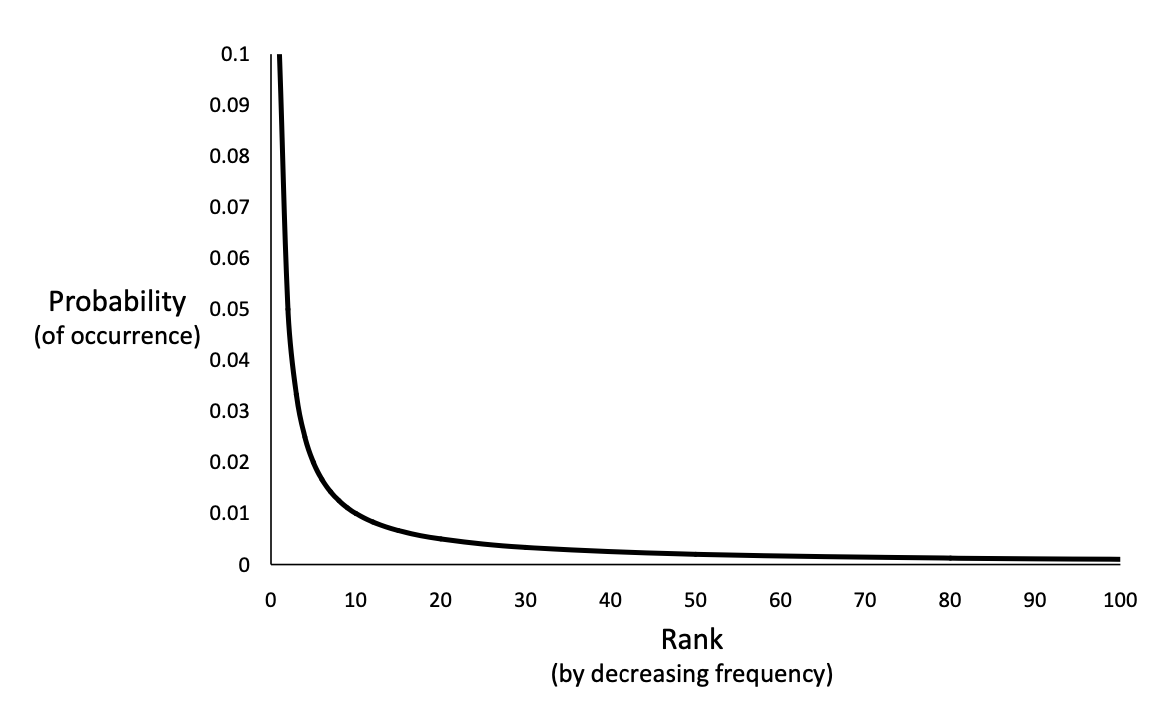
\includegraphics[scale=0.4]{figures/zipf.png}
%   \caption{Tradeoff tools KRR}
\end{minipage}
\vspace{0.35cm}

\textbf{Hapax Legomena}: words that occur once in a text corpus or book.
\\
\\
\textbf{\textcolor{NavyBlue}{Heaps' law}}: Relationship between size of corpus and size of vocabulary.
\\
\\
\begin{minipage}{.3\textwidth}
\centering
$v = k \cdot n^\beta$
\end{minipage}
\begin{minipage}{.7\textwidth}
v = vocabulary size for a corpus of size n words \\
$k$ and $\beta$ = parameters that vary for each collection.
\end{minipage}
\vspace{0.25cm}

\textbf{\textcolor{NavyBlue}{Heaps' law}} predicts that the number of new words will increase very rapidly when the corpus is small and will continue to increase indefinitely, but slower for larger corpora.
\newpage

Word occurrence statistics can also be used to estimate the size of the results from a web search. A \textbf{result} is any document (or web page) that contains all of the query words.  
\\
\\
If we assume that words occur \textbf{\textit{independently}} of each other, then the probability of a document containing all the words in the query is simply the \textbf{product of the probabilities} of the individual words occurring in a document. For example, if there are three query words a, b, and c, then:\\

\begin{minipage}{.4\textwidth}
% \centering
$P(a \cap b \cap c)=P(a) \cdot P(b) \cdot P(c)$
\end{minipage}
\begin{minipage}{.6\textwidth}
% \centering
$P(a \cap b \cap c)$ = \textcolor{Maroon}{joint probability}, or the probability that all three words occur in a document \\
\\
% \centering
$P(a), P(b), P(c)$ =  are the probabilities of each word occurring in a document.
\end{minipage}
\vspace{0.25cm}

A search engine will always have access to the number of documents that a word occurs in $\left(f_{a}, f_{b}\right.$, and $\left.f_{c}\right),$ and the number of documents in the collection $(N)$, so these probabilities can easily be estimated as $P(a)=$ $f_{a} / N, P(b)=f_{b} / N$, and $P(c)=f_{c} / N$:
$$f_{a b c}=N \cdot f_{a} / N \cdot f_{b} / N \cdot f_{c} / N=\left(f_{a} \cdot f_{b} \cdot f_{c}\right) / N^{2} \;\;\;\;\; \text{where $f_{abc}$: estimated size of result set.}$$

\textbf{\textcolor{Maroon}{But}}, this assumption does \textbf{not} lead to good estimates for result size, especially for \textbf{combinations} of \textbf{\textcolor{Maroon}{three words}}. The problem is that the words in these combinations do not occur independently of each other. If we see the word “fish” in a document, for example, then the word “aquarium” is more likely to occur in this document than in one that does not contain “fish”.
\\
\\
Better estimates are possible if \textbf{\textcolor{NavyBlue}{word co-occurrence}} information is also available. Obviously, this would give exact answers for two-word queries. For longer queries, we can improve the estimate by not assuming independence. In general, for three words:
\\

\begin{minipage}{.5\textwidth}
% \centering
$P(a \cap b \cap c)=P(a \cap b) \cdot P(c \mid(a \cap b))$
\end{minipage}
\begin{minipage}{.45\textwidth}
% \centering
$P(a \cap b)$ = probability that the words $a$ and $b$ \textcolor{NavyBlue}{co-occur} in a document \\
\\
$P(a), P(b), P(c)$ =  probability that the word $c$ occurs in a document given that the words $a$ and $b$ occur in the document.
\end{minipage}
\vspace{0.25cm}

These estimates are much better than the ones produced assuming independence, but they are \textbf{still too low}.
\\
\\
Skipped the last few paragraphs of 4.2, because I don't think this is very important.
\newpage

\subsection{Document Parsing}
\textbf{Document parsing} involves recognizing the content and structure of text document.
\\
\\
Metadata is information about a document that is not part of the text content. Metadata content includes document attributes such as date and author, and, most importantly, the \textbf{tags} that are used by \textbf{markup languages} to identify document components. Most popular are HTML and XML.
\\
\\
The \textbf{\textcolor{Red}{parser}} uses the \textbf{tags} and other metadata recognized in the document to interpret the document’s structure based on the syntax of the markup language (\textbf{\textcolor{NavyBlue}{syntactic analysis}}) and to produce a representation of the document that includes both the structure and content. 
\subsection{Tokenizing}
\textbf{\textcolor{Maroon}{Tokenizing}} is the process of forming words from the sequence of characters in a document. Some examples of issues involving tokenizing that can have significant impact on the effectiveness of search are:
\begin{itemize}
    \setlength\itemsep{0em}
    \item \textbf{Small words}: can be important in combination with other words. For example, master, world war II.
    \item \textbf{Hyphenated and non-hyphenated forms of words}
    \item \textbf{Special characters}: important part of the tags, URLs, code, and other important parts of documents that must be correctly tokenized.
    \item \textbf{Capitalized words}: can have different meaning from lowercase words. For ex- ample, “Bush” and “Apple”.
    \item \textbf{Apostrophes}
    \item \textbf{Numbers, including decimals}: for example, nokia 3250, quicktime 6.5 pro.
    \item \textbf{Periods can occur in numbers, abbreviations} (e.g., “I.B.M.”, “Ph.D.”), URLs, ends of sentences, and other situations.
\end{itemize}
\vspace{0.25cm}
Text processing for queries \textbf{\textcolor{Maroon}{must}} be the \textbf{same} as that used for documents. Otherwise, many of the index terms will simply not match the corresponding terms.

\subsection{Stopping}
Human language is filled with function words: words that have little meaning apart from other words. The most popular—“the,” “a,” “an,” “that,” and “those”—are determiners. These words are part of how we describe nouns in text, and express concepts like location or quantity. Prepositions, such as “over,” “under,” “above,” and “below,” represent relative position between two nouns.

In information retrieval, these function words have a second name: \textbf{\textcolor{NavyBlue}{stopwords}}. We call them \textcolor{NavyBlue}{stopwords} because text processing stops when one is seen, and they are thrown out. \textbf{Throwing out} these words \textbf{decreases index size}, \textbf{increases retrieval efficiency}, and generally \textbf{improves retrieval effectiveness}.
\\
\\
Constructing a stopword list must be done with \textbf{\textcolor{Red}{caution}}. Removing too many words will \textbf{\textcolor{Red}{hurt}} retrieval effectiveness.
\\
\\
If storage space requirements allow, it is best to at least index all words in the documents. If stopping is required, the stopwords can always be removed from queries. If keeping stopwords in an index is not possible because of space requirements, as few as possible should be removed in order to maintain maximum flexibility.

\subsection{Stemming}
\textbf{\textcolor{PineGreen}{Stemming}}, also called \textbf{\textcolor{PineGreen}{conflation}}, is a component of text processing that captures the relationships between different variations of a word. More precisely, \textbf{\textcolor{PineGreen}{stemming}} \textbf{reduces} the different forms of a word that occur because of \textbf{\textit{inflection}} (e.g., plurals, tenses) or \textbf{\textit{derivation}} (e.g., making a verb into a noun by adding the suffix -ation) to a common stem.
\\
\\
There are two basic types of \textbf{stemmers}: \textcolor{Maroon}{algorithmic} and \textcolor{NavyBlue}{dictionary}-based. An \textcolor{Maroon}{algorithmic} stemmer uses a small program to decide whether \textbf{two words} are \textbf{related}, usually based on knowledge of word suffixes for a particular language. By contrast, a \textcolor{NavyBlue}{dictionary}-based stemmer has no logic of its own, but instead \textbf{relies} on \textbf{pre-created dictionaries} of related terms to store term relationships.
\\

\begin{minipage}{.5\textwidth}
\textcolor{Maroon}{Algorithmic} stemmers:
\begin{itemize}
    \setlength\itemsep{0em}
    \item \textbf{Suffix-s stemmer}: assumes any word ending in the letter “s” is plural. Cakes $\rightarrow$ cake.
    \item \textbf{Porter stemmer}: consists of a number of steps, each containing a set of rules for removing suffixes. At each step, the rule for the longest applicable suffix is executed. 
\end{itemize}
\end{minipage}
\begin{minipage}{.5\textwidth}
\textcolor{NavyBlue}{Dictionary (Hybrid)}-based stemmers:
\begin{itemize}
    \setlength\itemsep{0em}
    \item \textbf{Krovetz stemmer}: makes constant use of a dictionary to check whether the word is valid. The Krovetz stemmer has the additional advan- tage of producing stems that, in most cases, are full words, whereas the Porter stemmer often produces stems that are word fragments.
\end{itemize}
\end{minipage}
\vspace{0.25cm}

Incorporating language-specific stemming algorithms is one of the most important aspects of customizing, or \textbf{\textcolor{Maroon}{internationalizing}}, a search engine for multiple languages.

\subsection{Phrases and N-grams}
A \textbf{\textcolor{Maroon}{phrase}} is equivalent to a simple \textbf{noun phrase}. This is often restricted even further to include just sequences of nouns, or adjectives followed by nouns. Phrases defined by these criteria can be identified using a \textbf{\textcolor{PineGreen}{part-of-speech (POS) tagger}}. A POS tagger marks the words in a text with labels corresponding to the part-of-speech of the word in that context. Taggers are based on statistical or rule-based approaches and are trained using large corpora that have been manually labeled.
\\
\\
\textbf{\textcolor{Maroon}{N-gram}}: any sequence of $n$ words. \\
\textbf{\textcolor{Maroon}{Unigram}}: single words. \\
\textbf{\textcolor{Maroon}{Bigrams}}: sequences of two words. \\
\textbf{\textcolor{Maroon}{Unigram}}: sequences of three words. \\
\\
The more frequently a word \textbf{\textcolor{Maroon}{N-gram}} occurs, the \textbf{more likely} it is to correspond to a \textbf{meaningful phrase in the language}. N-grams of all lengths form a Zipf distri- bution, with a few common phrases occurring very frequently and a large number occurring with frequency 1. In fact, the rank-frequency data for n-grams (which includes single words) fits the Zipf distribution better than words alone. 

\subsection{Ranking with indexes}
\textcolor{Maroon}{Unsorted arrays} are \textcolor{Maroon}{slow to search}, and \textcolor{RubineRed}{sorted arrays} are \textcolor{RubineRed}{slow at insertion}. By contrast, \textcolor{ForestGreen}{hash tables} and \textcolor{ForestGreen}{trees} are \textcolor{ForestGreen}{fast} for \textcolor{ForestGreen}{both search and insertion}. These structures are more complicated than arrays, but the speed difference is compelling.
\\
\\
\textbf{\textcolor{PineGreen}{Text search}} is very different from traditional computing tasks, so it calls for its own kind of data structure, the \textbf{\textcolor{BlueGreen}{inverted index}}.

\newpage
\subsection{Slides IR0 recap}
\textbf{Outline \textcolor{Maroon}{text analysis}}:
\begin{itemize}
    \setlength\itemsep{0em}
    \item[--] \textbf{Statistical properties of written text} (Zipf's law and Heaps' law)
    \item[--] \textbf{Text analysis pipeline}
    \begin{enumerate}
        \item Remove white-spaces and punctuation
        \item Convert terms to lower-case
        \item Remove stop-words
        \begin{itemize}
            \item[$\circ$] \textcolor{OrangeRed}{Frequency-based}: 
            \begin{itemize}
                \item Set a frequency threshold f
                \item Remove words with the frequency higher than f
            \end{itemize}
            \item[$\circ$] \textcolor{JungleGreen}{Dictionary-based}:
            \begin{itemize}
                \item Create a dictionary of stop-words
                \item Remove words that occur in this dictionary
            \end{itemize}
        \end{itemize}
        \item Convert terms to their stems
        \item Deal with phrases
        \item Apply language-specific processing rules
    \end{enumerate}
    \item[--] \textbf{Stemming}
    \begin{itemize}
        \item[$\circ$] \textcolor{Maroon}{Algorithmic}: Porter-stemmer
        \item[$\circ$] \textcolor{JungleGreen}{Dictionary-based}
        \begin{itemize}
            \item Large dictionary of related words
            \item Semi-automatic: run $\rightarrow$ running, runs, \textcolor{Red}{runned}, \textcolor{Red}{runly}
            \item New-words problem
        \end{itemize}
        \item[$\circ$] \textcolor{DarkOrchid}{Hybrid}: produces words, \textbf{not stems}. Comparable effectiveness with the Porter stemmer
        \begin{itemize}
            \item check the word in a dictionary, \textbf{if found}, leave it as is
            \item if not found, apply algorithmic stemming (remove suffixes)
            \item check the dictionary again
            \item if not found, apply rules to modify the ending
        \end{itemize}
    \end{itemize}
    \item[--] \textbf{Phrases}
    \begin{enumerate}
        \item detect noun phrases using a part-of-speech tagger
        \begin{itemize}
            \item sequences of nouns
            \item adjectives followed by nouns
        \end{itemize}
        \item Detect phrases at the query processing time \\
        Use index with word positions
        \item Use frequent \textbf{n-grams}, e.g., bigrams and trigrams
    \end{enumerate}
\end{itemize}

\newpage
\textbf{Outline \textcolor{Maroon}{indexing}}:
\begin{enumerate}
    \setlength\itemsep{0em}
    \item \textbf{Data structures}: Web Graph, Forward index, Page attribute file, Inverted index
    \item \textbf{Inverted index}
    \begin{enumerate}
        \item Dictionary
        \begin{itemize}
            \item Each entry contains
            \begin{itemize}
                \item Number of pages containing the term
                \item Pointer to the start of the inverted list
                \item Other meta-data about the term
            \end{itemize}
            \item B+ tree, hash table
        \end{itemize}
        \item Inverted lists
        \begin{itemize}
            \item Document identifiers
            \item Frequencies
            \item Positions
            \item Weights
        \end{itemize}
    \end{enumerate}
    \item \textbf{Constructing an index}
    \begin{itemize}
        \item Simple indexer \\
        \textbf{Problems} of this indexer:
        \begin{enumerate}
            \item In-memory:
            \begin{itemize}
                \item Two-pass index
                \item One-pass index with merging
            \end{itemize}
            \item Single-threaded
            \begin{itemize}
                \item Distributed indexing (MapReduce)
            \end{itemize}
        \end{enumerate}
    \end{itemize}
    \item \textbf{Updating an index} \\
    \textbf{Strategies}:
    \begin{itemize}
        \item No merge (low index maintenance cost, high query processing cost)
        \item Incremental update 
        \item Immediate merge (always a single index)
        \item Lazy merge (trade-off between index maintenance and query processing cost)
    \end{itemize}
    \textbf{Page deletions}:
    \begin{itemize}
        \item Maintain identifiers of deleted documents in memory, access during query processing
        \item Garbage collection (e.g., during index merging)
    \end{itemize}
\end{enumerate}
\newpage